\documentclass{standalone}
\usepackage{tikz}
\usetikzlibrary{arrows.meta, decorations.pathreplacing}
\begin{document}

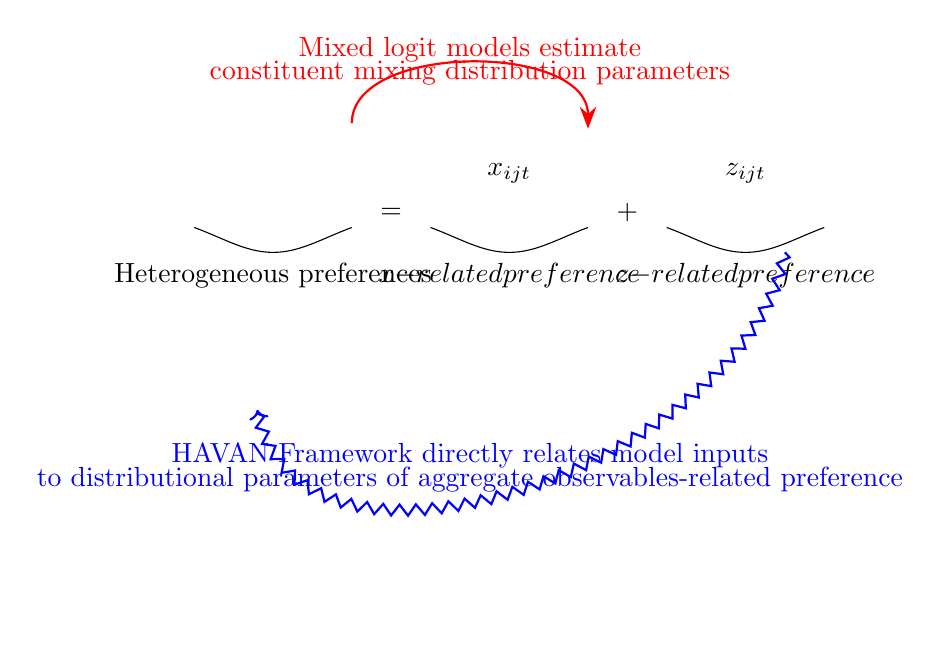
\begin{tikzpicture}[scale=1]
    % Colors
    \definecolor{myblue}{RGB}{0, 0, 255}
    \definecolor{myred}{RGB}{255, 0, 0}

    % Normal distributions
    \draw[domain=0:2, smooth, variable=\x, black] plot ({\x}, {-0.5*exp(-(\x-1)^2)});
    \node at (1, -0.8) {Heterogeneous preferences};

    \draw[domain=3:5, smooth, variable=\x, black] plot ({\x}, {-0.5*exp(-(\x-4)^2)});
    \node at (4, -0.8) {\( x\text{-related preference} \)};
    
    \draw[domain=6:8, smooth, variable=\x, black] plot ({\x}, {-0.5*exp(-(\x-7)^2)});
    \node at (7, -0.8) {\( z\text{-related preference} \)};

    % Equation symbols
    \node at (2.5, 0) {=};
    \node at (5.5, 0) {+};

    % Variables
    \node at (4, 0.5) {\( x_{ijt} \)};
    \node at (7, 0.5) {\( z_{ijt} \)};

    % Red curved arrow
    \draw[myred, thick, -{Stealth[scale=1.2]}, shorten >=2pt, shorten <=4pt] (2,1) to[out=90,in=90] (5,1);
    \node[myred, above] at (3.5, 1.8) {Mixed logit models estimate};
    \node[myred, above] at (3.5, 1.5) {constituent mixing distribution parameters};

    % Blue zigzag arrow
    \draw[myblue, thick, ->, decorate, decoration={zigzag, segment length=6pt, amplitude=2pt}] (7.5,-0.5) to[out=-100,in=-80] (0.8,-2.5);
    \node[myblue, below] at (3.5, -2.8) {HAVAN Framework directly relates model inputs};
    \node[myblue, below] at (3.5, -3.1) {to distributional parameters of aggregate observables-related preference};
\end{tikzpicture}

\end{document}